\section{Background}
\label{sec:Background}
\subsection{What is Blockchain?}
\label{subsection:WhatIsBlockchain}
Gartner\footnote{\url{https://www.gartner.com/}}, a research and advisory company, provides a yearly statistic called \quoteit{Hype Cycle for Emerging Technologies, 2017}. The y-axis shows the expectations in the technology and the x-axis the time. This is categorized into five sections:
\begin{enumerate*}[label={\arabic*)},font={\color{red!50!black}\bfseries}]
	\item Innovation Trigger
	\item Peak of Inflated Expectations
	\item Trough of Disillusionment
	\item Slope of Enlightenment
	\item Plateau of Productivity
\end{enumerate*}.  
\begin{figure}[!ht]
    \centering
    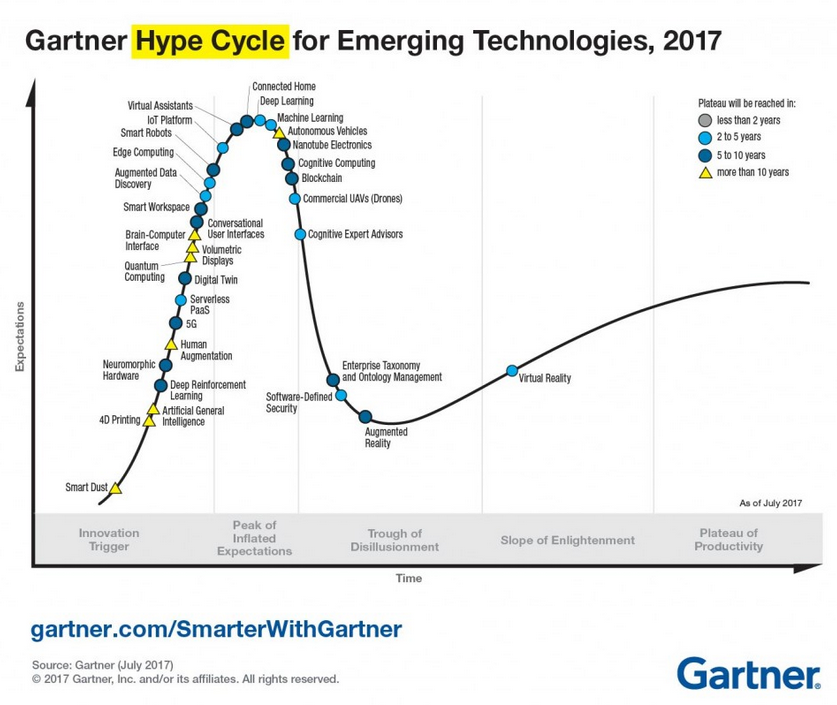
\includegraphics[width=0.6\textwidth]{gartner_hype_cycle.png}
    \label{gartner_hype_cycle}
    \caption{Gartner Hype Cycle for Emerging Technologies 2017}
\end{figure} \\
In 2016, the Blockchain technology was in the \quoteit{Peak of Inflated Expectations}. That means it gained a lot of publicity and produced several successful use cases, but also that not many firms took part in using this new technology. By 2017, the Blockchain moved into the area of \quoteit{Trough of Disillusionment}. This means that the interest in the technology is fading and that there is a certain number of use cases that did not succeed. The Blockchain is in between those two sections in 2017 and the final report of 2018 has not yet been published. \cite{2017_Panetta} \\
\begin{figure}[!ht]
    \centering
    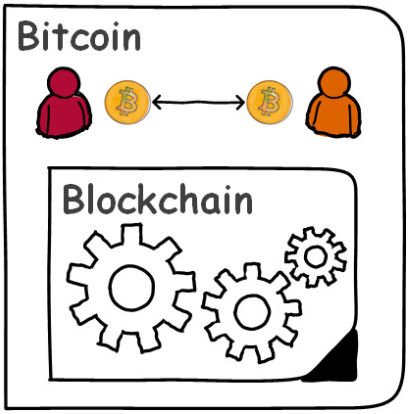
\includegraphics[width=0.20\textwidth]{blockchain_1.png}
    \label{blockchain_1}
    \caption{Bitcoin is not Blockchain}
\end{figure}
The main thing to mention here, is that the Blockchain is not the same as Bitcoin. Nevertheless, Blockchain started with the invention of Bitcoin by \citet{2009_Nakamoto} in 2009. Bitcoin is a system that used the Blockchain for digital payment processing. This makes Bitcoin the first application of the Blockchain technology. With the invention of Bitcoin, the following problems of cryptocurrencies were solved:
\begin{itemize}[noitemsep]
	\item Double spending problem (\quoteit{Byzantine Generals' Problem}\footnote{\url{https://en.wikipedia.org/wiki/Byzantine_fault_tolerance}})
	\item No trusted third-party
	\item Cryptographic proof instead of trust
\end{itemize}
The Blockchain is nothing less than a successful combination of already existing technologies. The technologies it combined are: 
\begin{enumerate*}[label={\arabic*)},font={\color{red!50!black}\bfseries}]
	\item Peer-to-Peer (P2P) networks \nomenclature[O]{P2P}{Peer-to-Peer Network}
	\item Cryptography
	\item Consensus decision-making
\end{enumerate*}.\\
A Peer-to-Peer (P2P) network is a form of a distributed architecture. Different peers participate in the system and all have equal rights. There is no central server, so the peers act as clients and servers at the same to share information between them. \cite{2001_Schollmeier}
Consensus decision-making is nothing less than a group decision-making process. Here, the group-members try to develop and then agree on a decision, which represents the best interest for the group. The consensus that they established can be seen the acceptable resolution.
Overall, Cryptography is the research field that tries to establish secure communication between peers when there is an enemy, in this field also called adversary, that could steal the information. So basically, it describes the practice of converting someone’s readable data, into unreadable data and vice-versa. \cite{2018_Meinel}
%______________________________________________________________________

\subsubsection{Consensus algorithms}
In a P2P Network, you have no trusted third party. Therefore, some rules need to be defined as for how to find a consensus between the different members of your system. There are multiple algorithms that already existed and are now used by various Blockchain technology implementations. Here, you can define between ‘mining’ and ‘minting’. In a mining process you focus on how many resources you spend to build a new block in the blockchain and in minting, you focus more on how much existing resources you have. Consensus algorithms using mining are for example Proof-of-Work (PoW), Proof-of-Burn (PoB). Proof-of-Stake (PoS), Delegated Proof-of-Stake and Federated Byzantine Agreement (FBA) are on the other hand example for algorithms using minting.
%______________________________________________________________________

\subsubsection{Public-key cryptography}
In the Blockchain context, Public-key cryptography is used. Every peer in the network has a private key and a public key. The public key can be seen by all other peers in the network, whereas the private key is kept secret by every user. The peers in the system have to fulfill two operations before sending a message: Encryption, Signature.
\begin{figure}[!ht]
    \centering
    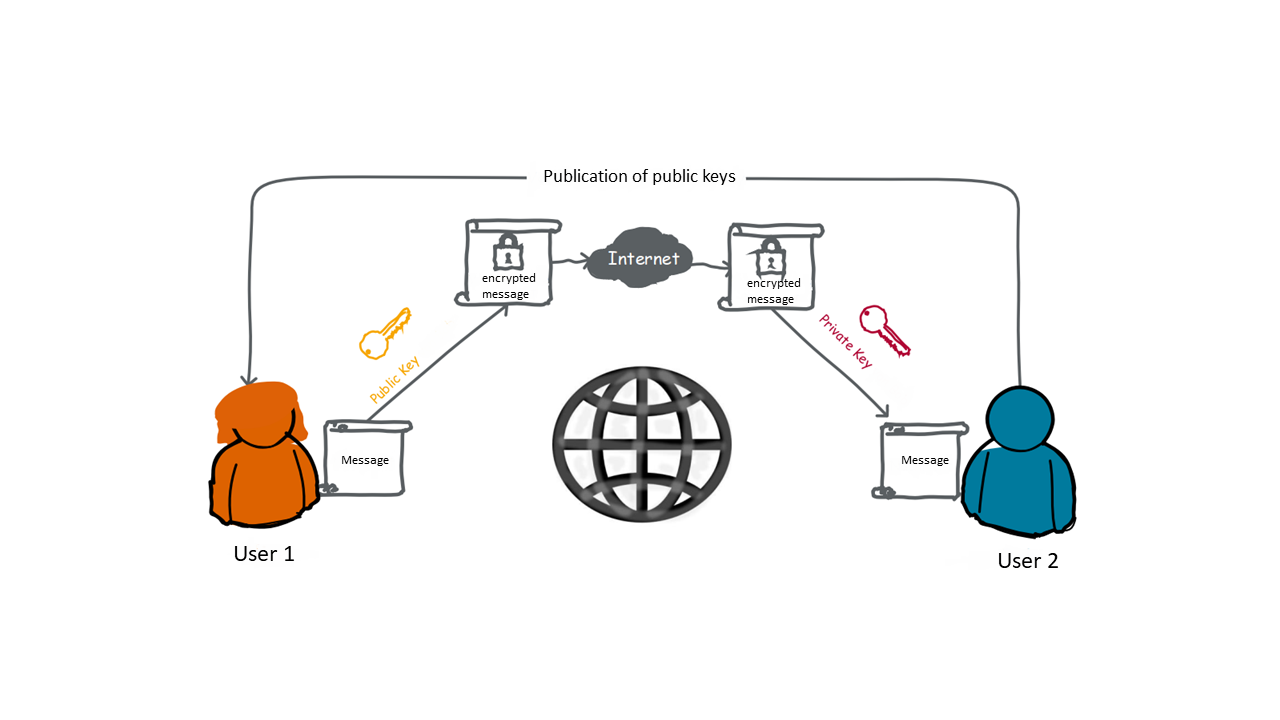
\includegraphics[width=0.8\textwidth]{encryption.png}
    \label{fig:encryption}
    \caption{Public-key cryptography: Encryption process}
\end{figure} \\
In the figure \ref{fig:encryption}, you can see that the user 1 wants to transfer a message to user 2, he encrypts the message using the public key of the user 2. The encrypted message is then transferred via internet, so the user 2 can see it. Since only he is in possession of his private key, he is the only one that is able to encrypt it and read the message that the user 1 wanted him to. All user that participate in the network have access to the public keys of the other peers, but only the peer with the right private key can encrypt the message that has been sent.\\
The signature process tries to copy a handwritten signature. This process provides proof, that a user is really the sender of a certain message. In Figure 4: Public-key cryptography: Signature Process, User 1 is sending a message to User 2. Since his message is very long, he is using a hash function to reduce the size of the message. Then he is using his private key to sign the message and the signed message will be send to another user. The user 2 then can verify with the public key of user 1, if it was really him that send the message. \\
\begin{figure}[!ht]
    \centering
    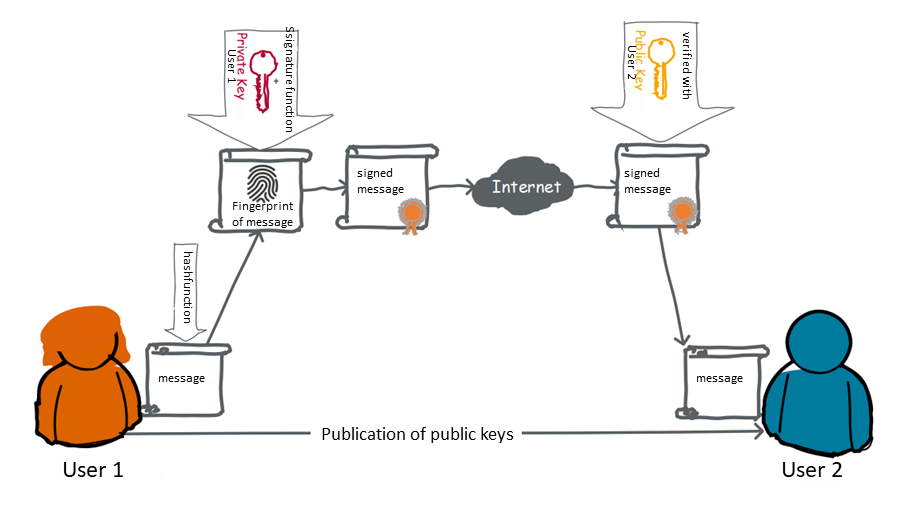
\includegraphics[width=0.8\textwidth]{signature.png}
    \label{fig:signature}
    \caption{Public-key cryptography: Signature Process}
\end{figure} \\
These two processes are combined in the Public-key cryptography process.\\
Further, I would like to explain a bit, what a cryptographic hash function is. The process is quite simple, you get an input of any size, which is sometimes also called a message, and you then use the hash function to map this input to an output of a fixed size. This function can not be reversed, meaning that you can not calculate the input by using the hash function on the output. In Blockchain systems, these hashes are organized into a hash tree or Merkle tree. This means that you have a certain number of transaction, that got hashed, then you hash them with each other and you build a tree until you arrive at the tree root, which is also called the Merkle Root. 

%______________________________________________________________________

\subsubsection{Types of Blockchains}
There is not a general specification of the different types of blockchains. Nevertheless, some researches are trying to establish a common standard. \cite{2018_Fernandez} mention that there are public and private Blockchains. Anyone can use a public blockchain without the approval of third parties, but a private blockchain is controlled by someone that can allow other peers to join the ecosystem. There are also permissionless and permissioned blockchains. The difference between those is that in a permissionless environment, any peer can act as a normal user or a miner and has access to all the functionalities offered by the blockchain. A permissioned blockchain is controlled by one instance and they can authorize peers to have access to certain functionalities and deny them the access to others. Another term is a consortium Blockchain. Here certain predefined peers have the control over the consensus process. \cite{2018_Meinel}
They also differ between logic-oriented and transaction oriented blockchains. Logic-oriented solutions focus on executing a certain logic implemented, like for example the smart contracts of Ethereum. The Bitcoin Blockchain is an example for a transaction oriented blockchain because it is clearly focused on transferring the cryptocurrency. Also, a blockchain system can be token-based or not.

%______________________________________________________________________

\subsubsection{Hyperledger}
In the beginning, the ‘Hyperledger’ project was conducted by 11 different groups, including the Linux Foundation, IBM, JP Morgan and many more. Since this project is open source, the number of collaborators is constantly growing. Currently they have already developed various tools for their Hyperledger Fabric Blockchain. Their goal by implementing this blockchain technology was to provide an open source blockchain for enterprises so that they can construct industry-specific systems for secure transaction handling.

%______________________________________________________________________

\clearpage
\import{sections/}{subsec_blockchain_reviews.tex}